\documentclass[a4paper,11pt]{book}
\usepackage[francais]{babel}
\usepackage[table]{xcolor}
\usepackage{amsmath}
\usepackage[utf8]{inputenc}
\usepackage{textcomp}
\usepackage{gensymb}
%\usepackage[francais]{babel}
\usepackage[T1]{fontenc}
\usepackage{makeidx}
\usepackage{graphicx}
\usepackage{enumitem}
\usepackage{float}
\usepackage{relsize}
\usepackage{amsmath,amsfonts,amssymb}
\usepackage{multirow}
\usepackage{layout}
\usepackage{amsthm}
\usepackage{lmodern}
\usepackage{fancyhdr}
\usepackage{enumitem}
\usepackage{geometry}
\usepackage{listings}
\usepackage{eso-pic}


\lstdefinestyle{generalFrame}{
aboveskip=3mm,
belowskip=-2mm,
basicstyle=\footnotesize,
breakatwhitespace=false,
breaklines=true,
captionpos=b,
commentstyle=\color{red},
deletekeywords={...},
escapeinside={\%*}{*)},
extendedchars=true,
framexleftmargin=16pt,
framextopmargin=3pt,
framexbottommargin=6pt,
frame=tb,
keepspaces=true,
keywordstyle=\color{blue},
language=Python,
literate=
{²}{{\textsuperscript{2}}}1
{⁴}{{\textsuperscript{4}}}1
{⁶}{{\textsuperscript{6}}}1
{⁸}{{\textsuperscript{8}}}1
{€}{{\euro{}}}1
{é}{{\'e}}1
{è}{{\`{e}}}1
{ê}{{\^{e}}}1
{ë}{{\¨{e}}}1
{É}{{\'{E}}}1
{Ê}{{\^{E}}}1
{û}{{\^{u}}}1
{ù}{{\`{u}}}1
{â}{{\^{a}}}1
{à}{{\`{a}}}1
{á}{{\'{a}}}1
{ã}{{\~{a}}}1
{Á}{{\'{A}}}1
{Â}{{\^{A}}}1
{Ã}{{\~{A}}}1
{ç}{{\c{c}}}1
{Ç}{{\c{C}}}1
{õ}{{\~{o}}}1
{ó}{{\'{o}}}1
{ô}{{\^{o}}}1
{Õ}{{\~{O}}}1
{Ó}{{\'{O}}}1
{Ô}{{\^{O}}}1
{î}{{\^{i}}}1
{Î}{{\^{I}}}1
{í}{{\'{i}}}1
{Í}{{\~{Í}}}1,
morekeywords={*,...},
numbers=none,
numbersep=10pt,
numberstyle=\tiny\color{black},
rulecolor=\color{black},
showspaces=false,
showstringspaces=false,
showtabs=false,
stepnumber=1,
stringstyle=\color{gray},
tabsize=4,
title=\lstname,
}

\definecolor{darkwhite}{rgb}{0.94,0.94,0.94}
\definecolor{darkseagreen}{rgb}{0.56, 0.74, 0.56}
\definecolor{darkpastelblue}{rgb}{0.47, 0.62, 0.8}

\lstnewenvironment{mypython}
  {\lstset{language=Python,
  style =generalFrame,
  backgroundcolor=\color{darkwhite} }}
  {}

\lstnewenvironment{mybash}
  {\lstset{language=bash,
  	style=generalFrame,
	backgroundcolor=\color{darkseagreen} }}
  {}

\lstnewenvironment{myoutput}
  {\lstset{language=bash,
  	style=generalFrame,
	backgroundcolor=\color{darkpastelblue} }}
  {}


\geometry{hmargin=2.2cm,vmargin=2.9cm}

 
\pagestyle{fancy}
\fancyhf{}
\fancyhead[L]{\leftmark}
\fancyfoot[C]{\thepage}
    

\def\entetehpos{-50}
\def\entetevpos{540}

\newcommand{\HRule}{\rule{\linewidth}{0.5mm}}


\newcommand{\blap}[1]{\vbox to 0pt{#1\vss}}
\newcommand\AtUpperLeftCorner[3]{%
\put(\LenToUnit{#1},\LenToUnit{\dimexpr\paperheight-#2}){\blap{#3}}%
}
\newcommand\AtUpperRightCorner[3]{%
\put(\LenToUnit{\dimexpr\paperwidth-#1},\LenToUnit{\dimexpr\paperheight-#2}){\blap{\llap{#3}}}%
}

\setlength{\headheight}{15.35403pt}
\begin{document}
\frontmatter

%==============================
%	PAGE DE GARDE
%==============================

%%%% Ancienne Version (use Package PageDeGarde)
%\let\cleardoublepage\clearpage
%\title{ \usefont{T1}{ptm}{m}{n} Tutoriel TensorFlow}

%\annee{2017-2018}

%\Auteur{IKNI Layachi}{}

%\Encadrant{Pag\'e Vincent}{MCF à l'Université des Antilles}

%	Nouvelle version
\begin{titlepage}
	\AddToShipoutPicture{
		\AtUpperLeftCorner{1.5cm}{1cm}{
\includegraphics[height=3cm]{figures/logo_ua_0.jpg}}
		\AtUpperRightCorner{1.5cm}{1cm}{
\includegraphics[height=3cm]{figures/banniere_lamia.png}}
	}
  \begin{sffamily}
  \begin{center}
	~\\[4cm]

    % Title
    \HRule \\[0.4cm]
    { \huge \bfseries Tutoriel TensorFlow\\[0.4cm] }


    
\includegraphics[width=10cm]{figures/logoTensorFlow.png}
    \HRule \\[6cm]


    % Author and supervisor
	
    \begin{minipage}{0.8\textwidth}
      \begin{flushleft} \large
        IKNI \textsc{Layachi}\\
        PAG\'E \textsc{Vincent}\\
      \end{flushleft}
    \end{minipage}
    \vfill    
    % Bottom of the page
    {\large 1\ier{} janvier 2018}
  \end{center}
  \end{sffamily}
\end{titlepage}
\ClearShipoutPicture

%\maketitle

%\newpage
%\section*{Remerciements}
%\bigskip
%\pagestyle{plain}
%\bigskip
%\newpage 

\newpage
\tableofcontents

\mainmatter
\chapter{Introduction }


\section{Installation}
TensorFlow est une librairie de calcul dédiée à l'apprentissage automatique. On peut l'utiliser avec python, java, C,.... Dans notre cas, nous utiliserons python.


Pour l'installation, nous avons suivi les instructions du tutoriel officiel qui se trouve ici, sans difficultés :

https://www.tensorflow.org/install/


\section{Présentation TensorFlow et TensorBoard}

\subsection{Premiers concepts de TensorFlow}

Tout d'abord, on peut utiliser TensorFlow de deux façons :
\begin{itemize}
\item En utilisant des algorithmes précodés, utilisant la classe \textbf{Estimator}
\item En maitrisant chaque étape du calcul.
\end{itemize}

Dans le second cas, il est nécessaire de comprendre que TensorFlow
s'appuie sur des concepts de programmation très différents d'une programmation standard python.

Pour bien comprendre ces concepts, prenons un exemple :
On veut que notre programme prenne une valeur réelle (x), calcule une valeur  $y = W*x+b$ avec $W$ et $b$ des valeurs réelles que notre programme sera appelé à modifier plus tard.

Le code correspondant en python est le suivant
\begin{mypython}
x = 2
W = 0.3
b = -0.3
y = W*x+b
print(y)
\end{mypython}

La sortie de ce programme serait :
\begin{myoutput}
0.3
\end{myoutput}

ici, $W$, $b$ , $x$ et $y$ sont des variables du programmes.
Néanmoins, dans le contexte de notre programme, elles jouent des rôles très différents :
\begin{itemize}
\item $x$ est une entrée 
\item $W$ et $b$ sont des valeurs modifiables
\item $y$ est calculé à partir de $x$, $W$ et $b$
\end{itemize}

La programmation en TensorFlow, met en place cette différence.
\begin{itemize}
\item $x$ sera appelé un \textbf{placeholder} , (en deux mots : une variable dont on promet qu'on lui donnera une valeur au moment du run)
\item $W$ et $b$ seront définis comme des variables
\item $y$ sera défini implicitement par l'équation de calcul 
\end{itemize}

Notons qu'il existe aussi la notion de constante, non présentée ici, mais facile a appréhender.

Le code correspondant en TensorFlow est le suivant :
\begin{mypython}
import tensorflow as tf

x = tf.placeholder(tf.float32)

W = tf.Variable([.3], dtype=tf.float32)
b = tf.Variable([-.3], dtype=tf.float32)

y = W*x + b

print(y)
\end{mypython}

La sortie de ce programme est alors surprenante :
\begin{myoutput}
Tensor("add:0", dtype=float32)
\end{myoutput}

De fait, nous n'avons pas calculé la valeur de $y$.\\
En fait notre programme ne manipule pas des variables au sens traditionnel, mais explique les dépendances entres les différents éléments de notre programme (ce sont des nœuds du graphes de calcul). TensorFlow s'appuie sur ce graphe de calcul, sur lequel nous reviendrons plus tard pour comprendre son intérêt.\\

Le graphe correspondant est représenté ci-dessous pour information.
\begin{figure}[H]

\begin{center}
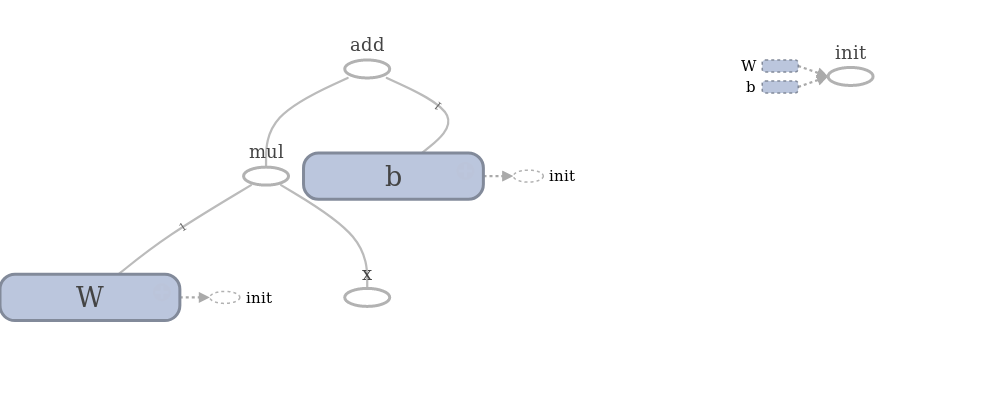
\includegraphics[width=10cm]{./figures/graphAddition.png} 
\end{center}
\caption{Graphe de calcul simple}
\end{figure}

On retrouve dans ce graphes la présence des deux variables ($W$ et $b$), le placeholder $x$, et un noeud $add$ dont la sortie correspond à $y$.


Par ailleurs, les variables au sens TensorFlow sont des nœuds de calculs qui peuvent être modifiés. Elle ne sont pas initialisées par leur déclaration. Il faudra explicitement demander leur initialisation pour qu'elles agissent comme on s'y attend.
Il s'agit maintenant pour que notre programme calcule bien la valeur voulue de :
\begin{itemize}
\item construire le graphe de calcul a partir des informations précédentes.
\item initialiser les variables $W$ et $b$
\item lancer le calcul de y avec une valeur choisie pour $x$...
\end{itemize}

Ajoutons les codes suivants à notre programme
\begin{mypython}
sess = tf.Session()
\end{mypython}
Le code ci-dessus construit le graphe.
\begin{mypython}
init = tf.global_variables_initializer()
sess.run(init)
\end{mypython}
Le code ci-dessus initialise toutes les variables du programme (W et b). En fait, ce code construit un noeud de calcul correspondant a l'initialisation (première ligne) et lance le calcul correspondant (deuxième ligne).

\begin{mypython} 
resu = sess.run(y, {x:2}) 
print(resu)
\end{mypython}
Ce code lance le calcul de y, en prenant soin de placer la valeur 2 dans le placeholder x et afficher le résultat attendu
\begin{myoutput}
[0.3]
\end{myoutput}
Pour comprendre l'intérêt de ces concepts de graphe de calcul, ajoutons à la fin de notre programme existant le code suivant :

\begin{mypython} 
resu = sess.run(y, {x:[1, 2, 3]}) 
print(resu)
\end{mypython} 

Cette fois ci, les sorties sont :

\begin{mypython} 
[0.3]
[0.  0.3 0.6]
\end{mypython} 

Nous avons en fait lancé deux runs (deux calculs de y). La première fois, x est un réel, la seconde fois x est un tableau de réels. Dans le second cas, pour chaque valeur de x, une valeur est calculée pour y.
Notre programme a donc mis en place une procédure de calcul (le graphe de calcul) que l'on peut utiliser de multiples fois, avec différentes valeurs d'entrées (qui de plus prennent des formes différentes).
Une grande partie de la force de TensorFlow tient dans ces notions.
Voici donc le code du programme complet :

\begin{mypython} 
import tensorflow as tf

x = tf.placeholder(tf.float32, name="x")

W = tf.Variable([.3], dtype=tf.float32, name="W")
b = tf.Variable([-.3], dtype=tf.float32, name="b")

y = W*x + b

print(y)

sess = tf.Session()

init = tf.global_variables_initializer()
sess.run(init)

resu = sess.run(y, {x:2}) 
print(resu)

resu = sess.run(y, {x:[1, 2, 3]}) 
print(resu)
\end{mypython} 

\subsection{Premiers pas avec Tensorboard}

TensorBoard est l'outil de visualisation associé à TensorFlow. Il permet de visualiser le graphe de calcul, mais aussi des valeurs importantes retenues lors des calculs exécutés sur ce graphe de calcul.
Pour sélectionner les informations a visualiser, nous l'indiquerons a notre programme TensorFlow. Le programme sauvegardera ces informations dans un répertoire spécifique.

On pourra alors lancer l'exécutable TensorBoard qui va analyser ce répertoire, créer un serveur web local que l'on pourra consulter pour visualiser nos informations...
Voyons comment tout ceci se fait.


Ajout de code dans le programme TensorFlow (a la fin du programme précédent) :
\begin{mypython}
pathLog="./pathLog/";
writer = tf.summary.FileWriter(pathLog, sess.graph)
writer.close()
\end{mypython}
Ici, on choisit le répertoire (répertoire de Log) dans lequel seront stockées les informations importantes, et on crée un objet permettant d'écrire les informations de notre programme sur le disque. Ici, nous ne sauvons que le graphe de calcul. Enfin, on ferme cet objet.
On lance notre programme TensorFlow 
\begin{mybash}
python .\premiersPas.py
\end{mybash}
On lance ensuite TensorBoard sur le répertoire de Log avec une ligne dépendant de l'OS utilisé :

Sous windows :
\begin{mybash}
tensorboard.exe --logdir=./pathLog
\end{mybash}
Sous linux :
\begin{mybash}
tensorboard --logdir=./pathLog
\end{mybash}

L’exécution donne le message suivant :
\begin{myoutput}
Starting TensorBoard b'41' on port 6006
(You can navigate to http://127.0.1.1:6006)
\end{myoutput}


Enfin, on ouvre un navigateur dans lequel on indique l'URL de consultation indiquée par la sortie précédente.

Voici une capture de la visualisation obtenue :
\begin{figure}[H]

\begin{center}
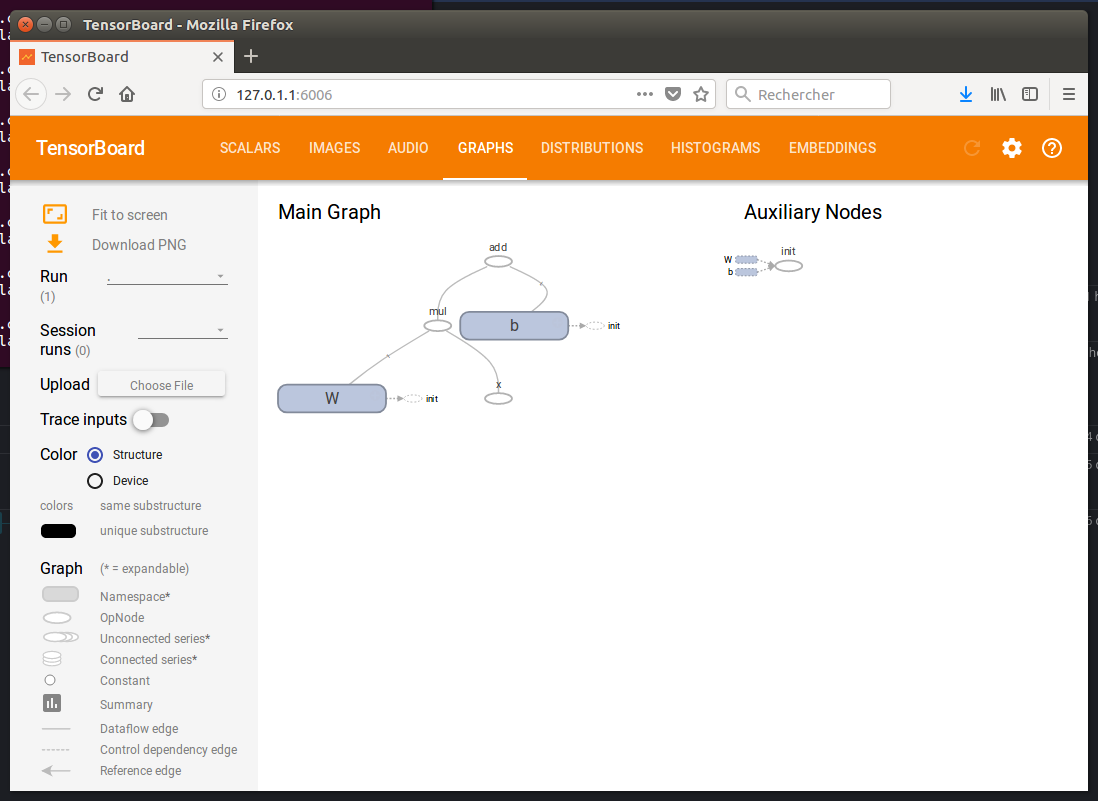
\includegraphics[width=10cm]{./figures/premierTensorBoard.png} 
\end{center}
\caption{La fenêtre de visualisation de TensorBoard}
\end{figure}

On retrouve ici le graphe précédent. Notez le sous graphe en haut a droite (noeud init) correspondant à l'initialisation des variables dont nous avons parlé précédemment. 

\chapter{Premier apprentissage automatique : Régression Linéaire}

\section{Codage de la Régression Lineaire manuelle}
Il s'agit du problème classique de régression linéaire. on se donne un ensemble de valeurs de $x$, et un ensemble de valeurs attendues pour chacun de ces $x$. L'objectif est de trouver la droite qui passe le plus près de tous ces points.
\begin{mypython}
import tensorflow as tf

x = tf.placeholder(tf.float32)
sortieVoulue = tf.placeholder(tf.float32)

W = tf.Variable([.3], dtype=tf.float32)
b = tf.Variable([-.3], dtype=tf.float32)

sortieCalculee = W*x + b
\end{mypython}
Nous avons bien défini nos entrées :
\begin{itemize}
\item $x$ : un placeholder dans lequel nous placerons au moment du run les abscisses des points
\item $y$ : un placeholder dans lequel nous placerons au moment du run les ordonnées des points
\end{itemize}

Par ailleurs, nous allons chercher des droites, qui sont paramétrées par leur pente $W$ et leur abscisse à l'origine $b$. Nous avons fixé les valeurs initiales de $W$ et $b$ a respectivement 0.3 et -0.3. Pour un couple $(W,b)$, nous avons une droite qui à $x$ associe $sortieCalculee$.
Notre problème consiste donc a modifier $W$ et $b$ pour que $sortieCalculee$ soit aussi prêt que possible de $sortieVoulue$.
Pour un couple $(W,b)$, évaluons l'erreur que l'on commet. on peut mesurer la somme des erreurs quadratiques sur chaque entrée :

\begin{mypython}
squared_deltas = tf.square(sortieCalculee - sortieVoulue)
erreur = tf.reduce_sum(squared_deltas)
\end{mypython}
Ajoutons enfin le run qui permettra de faire ces calculs pour les valeurs initiales de W et b :
\begin{mypython}
sess = tf.Session()

init = tf.global_variables_initializer()
sess.run(init)

print("erreur :",sess.run(erreur,{x: [1, 2, 3, 4], sortieVoulue: [0, -1, -2, -3]}))
\end{mypython}
Pour nos valeurs initiales, l'erreur totale est donnée par la sortie suivante
\begin{myoutput}
erreur : 23.66
\end{myoutput}
De fait, quelques calculs rapides permettrait de trouver les meilleures valeurs possible de W,b : (-1, 1). Dans le cas particulier des x et sortieVoulue donnés, il existe réellement une droite qui passe par ces points...

Essayons de vérifier cela 
\begin{mypython}
fixW = tf.assign(W, [-1.])
fixb = tf.assign(b, [1.])
sess.run([fixW, fixb])

print("erreur :",sess.run(erreur,{x: [1, 2, 3, 4], sortieVoulue: [0, -1, -2, -3]}))
\end{mypython}
Les deux premières lignes créent chacune un noeud dont l'objectif est de corriger les valeurs de $W$ et $b$. La troisième ligne lance le calcul sur ces nœuds, modifiant ainsi les valeurs de nos variables
Enfin la dernière ligne calcule l'erreur pour les $x$ et $sortieVoulue$ fournis avec le résultat suivant :
\begin{myoutput}
erreur : 0.0
\end{myoutput}
Essayons maintenant de trouver automatiquement ces valeurs pour W et b :
\begin{mypython}
optimizer = tf.train.GradientDescentOptimizer(0.01)
train = optimizer.minimize(erreur)

sess.run(init) # reset values to incorrect defaults.
for i in range(1000):
  sess.run(train, {x: [1, 2, 3, 4], sortieVoulue: [0, -1, -2, -3]})

print("(W,b finaux) :", sess.run([W, b]))
\end{mypython}
Pour cela, nous utilisons un objet \textbf{optimizer} prédéfini par TensorFlow, et qui opérera une descente de gradient (avec un pas de 0.0.1). On définit un nœud de calcul (train) dont le but est de minimiser  l'erreur.
La ligne suivante réinitialise les valeurs de $W$ et $b$ à (0.3, -0.3)
puis, 1000 fois de suite, on calcule le nœud train. Chaque itération améliore un peu les valeurs $(W et b)$. Il faut noter que nulle part, on ne spécifie que les valeurs à modifier sont $W$ et $b$... le programme le devine à partir du graphe : $W$ et $b$ sont les seules variables du graphe....
Enfin la dernière ligne affiche les valeurs finales trouvées :
\begin{myoutput}
(W,b finaux):[array([-0.9999969], dtype=float32), array([0.9999908], dtype=float32)]
\end{myoutput}

On voit que notre programme a trouvé pour $W$ et $b$ des valeurs très proches des valeurs cherchées (-1,1)
Voici donc le code complet de ce programme
\begin{mypython}
import tensorflow as tf

W = tf.Variable([.3], dtype=tf.float32, name="W")
b = tf.Variable([-.3], dtype=tf.float32, name="b")
x = tf.placeholder(tf.float32, name="x")
sortieCalculee = W*x + b

sortieVoulue = tf.placeholder(tf.float32, name="sortieVoulue")

squared_deltas = tf.square(sortieCalculee - sortieVoulue)
erreur = tf.reduce_sum(squared_deltas)


sess = tf.Session()


init = tf.global_variables_initializer()
sess.run(init)


print(sess.run(sortieCalculee, {x: [1, 2, 3, 4]}))

print("erreur totale :", sess.run(erreur, {x: [1, 2, 3, 4], sortieVoulue: [0, -1, -2, -3]}))


fixW = tf.assign(W, [-1.])
fixb = tf.assign(b, [1.])
sess.run([fixW, fixb])

print("erreur totale :", sess.run(erreur, {x: [1, 2, 3, 4], sortieVoulue: [0, -1, -2, -3]}))


optimizer = tf.train.GradientDescentOptimizer(0.01)
train = optimizer.minimize(erreur)

sess.run(init) # reset values to incorrect defaults.
for i in range(1000):
  sess.run(train, {x: [1, 2, 3, 4], sortieVoulue: [0, -1, -2, -3]})

print("(W,b finaux) :", sess.run([W, b]))

pathLog="./pathLog/";
writer = tf.summary.FileWriter(pathLog, sess.graph)
writer.close()
\end{mypython}
Voici également le graphe de calcul que notre programme a utilisé
\begin{figure}[H]

\begin{center}
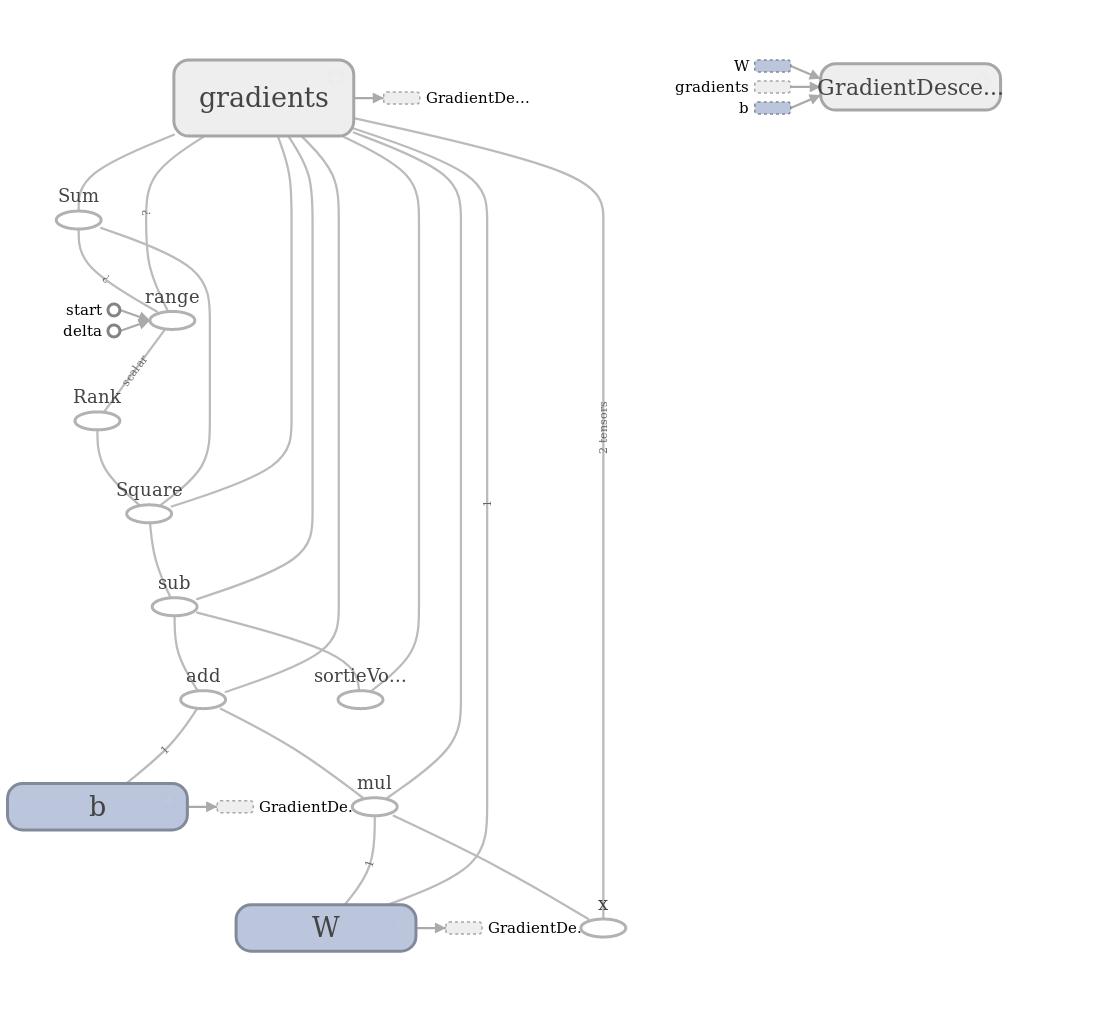
\includegraphics[width=10cm]{./figures/graphRegressionLineaire.png} 
\end{center}
\caption{Graphe de calcul pour la régression linéaire}
\end{figure}

En l'état, une partie de ce graphe est facile a expliquer (en bas a gauche), le reste est assez... mystérieux mais est clairement associé a la descente du gradient...

\section{Suivi de performance dans TensorBoard}
Nous voulons suivre l’évolution de l'erreur au cours de l'apprentissage des $W$,$b$ du programme précédent et la visualiser à l'aide de TensorBoard.
Il va falloir modifier notre programme TensorFlow pour logger cette erreur. Les lignes à insérer étant réparties un peu partout, nous indiquerons chaque modification séparément et fourniront le code complet en fin de section.

Tout d'abord, il faut signaler que l'on s'intéresse à l'erreur. Ceci est fait par la ligne suivante :
\begin{mypython}
tf.summary.scalar('erreur quadratique', erreur)
\end{mypython}
De ce que nous avons compris, on peut s’intéresser à plusieurs paramètres, et il faudra les fusionner pour les logger avec la ligne suivante :
\begin{mypython}
merged = tf.summary.merge_all()
\end{mypython}
Lors de chaque run, pendant l’entraînement, il faudra demander le calcul de ce merged. Enfin, le résumé devra être sauvé grâce au writer de TensorBoard... 
\begin{mypython}
for i in range(1000):
  summary, _ = sess.run([merged,train], {x: [1, 2, 3, 4], sortieVoulue: [0, -1, -2, -3]})
  writer.add_summary(summary, i)
\end{mypython}
Si une partie des notions utilisées ici nous échappe, voici néanmoins un code complet, fonctionnel :
\begin{mypython}
import tensorflow as tf

## Définition des variables 
W = tf.Variable([.3], dtype=tf.float32, name="W")
b = tf.Variable([-.3], dtype=tf.float32, name="b")
x = tf.placeholder(tf.float32, name="x")
sortieCalculee = W*x + b

sortieVoulue = tf.placeholder(tf.float32, name="sortieVoulue")

squared_deltas = tf.square(sortieCalculee - sortieVoulue)
erreur = tf.reduce_sum(squared_deltas)


optimizer = tf.train.GradientDescentOptimizer(0.01)
train = optimizer.minimize(erreur)

sess = tf.Session()

# Configuration de TensorBoard
pathLog="./pathLog/";
writer = tf.summary.FileWriter(pathLog, sess.graph)
tf.summary.scalar('erreur quadratique', erreur)
#tf.summary.scalar('W', W)
merged = tf.summary.merge_all()

init = tf.global_variables_initializer()
sess.run(init) # reset values to incorrect defaults.
for i in range(1000):
  summary, _ = sess.run([merged,train], {x: [1, 2, 3, 4], sortieVoulue: [0, -1, -2, -3]})
  writer.add_summary(summary, i)
  
print("(W,b finaux) :", sess.run([W, b]))


writer.close()
\end{mypython}

Voici le résultat final visualisé dans TensorBoard
\begin{figure}[H]

\begin{center}
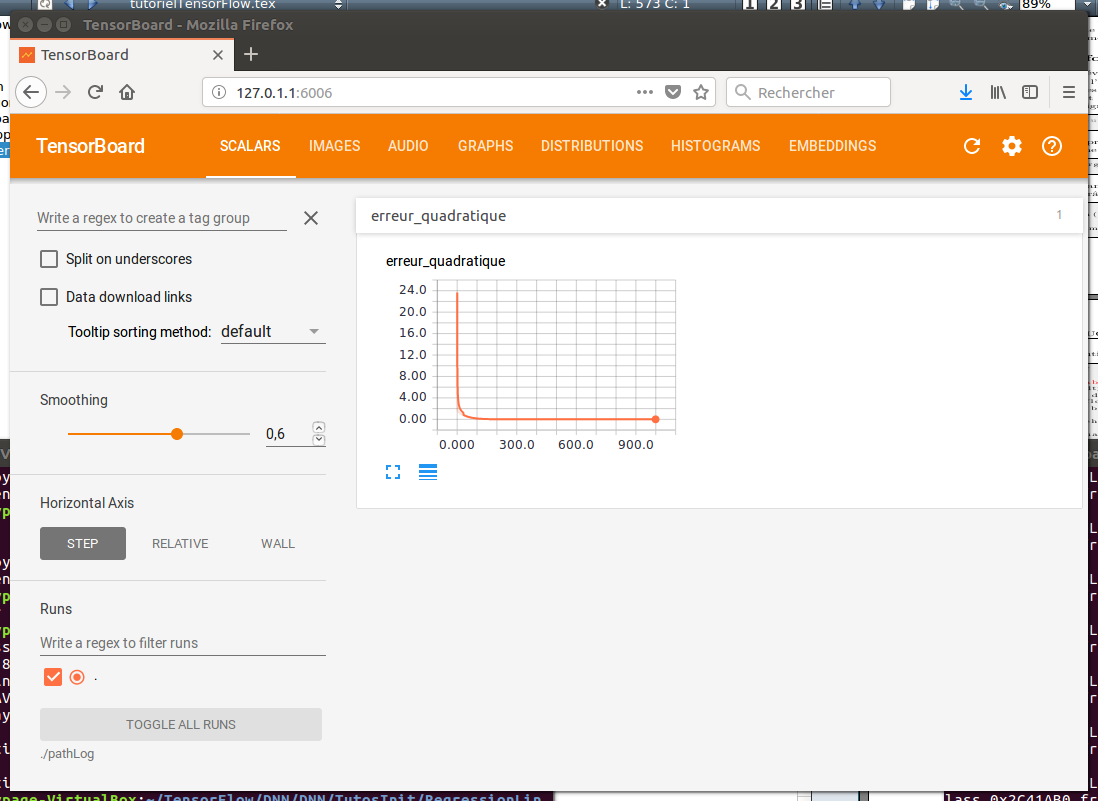
\includegraphics[width=10cm]{./figures/TBScalarRegression.png} 
\end{center}
\caption{Visualisation de l'évolution de l'erreur lors de l'apprentissage}
\end{figure}

\section{Régression Linéaire avec TfEstimator}

tf.estimator est une bibliothèque TensorFlow de haut niveau qui simplifie la mécanique de l'apprentissage automatique, notamment:
\begin{itemize}
\item exécuter des boucles d'entraînement
\item exécuter des boucles d'évaluation
\item gérer des ensembles de données
\end{itemize}

tf.estimator définit de nombreux modèles courants.
Utilisons le ici pour le problème précédent de régression linéaire
\begin{mypython}
# NumPy is often used to load, manipulate and preprocess data.
import numpy as np
import tensorflow as tf

# Declare list of features. We only have one numeric feature. There are many
# other types of columns that are more complicated and useful.
feature_columns = [tf.feature_column.numeric_column("x", shape=[1])]

# An estimator is the front end to invoke training (fitting) and evaluation
# (inference). There are many predefined types like linear regression,
# linear classification, and many neural network classifiers and regressors.
# The following code provides an estimator that does linear regression.
estimator = tf.estimator.LinearRegressor(feature_columns=feature_columns)

# TensorFlow provides many helper methods to read and set up data sets.
# Here we use two data sets: one for training and one for evaluation
# We have to tell the function how many batches
# of data (num_epochs) we want and how big each batch should be.
x_train = np.array([1., 2., 3., 4.])
y_train = np.array([0., -1., -2., -3.])
x_eval = np.array([2., 5., 8., 1.])
y_eval = np.array([-1.01, -4.1, -7, 0.])

input_fn = tf.estimator.inputs.numpy_input_fn(
    {"x": x_train}, y_train, batch_size=4, num_epochs=None, shuffle=True)

train_input_fn = tf.estimator.inputs.numpy_input_fn(
    {"x": x_train}, y_train, batch_size=4, num_epochs=1000, shuffle=False)

eval_input_fn = tf.estimator.inputs.numpy_input_fn(
    {"x": x_eval}, y_eval, batch_size=4, num_epochs=1000, shuffle=False)

# We can invoke 1000 training steps by invoking the  method and passing the
# training data set.
estimator.train(input_fn=input_fn, steps=1000)

# Here we evaluate how well our model did.
train_metrics = estimator.evaluate(input_fn=train_input_fn)
eval_metrics = estimator.evaluate(input_fn=eval_input_fn)

print("train metrics: %r"% train_metrics)
print("eval metrics: %r"% eval_metrics)
\end{mypython}

Le code est relativement simple. On peut noter que :
\begin{itemize}
\item on ne construit plus le graphe nous même
\item On ne lance plus de run manuellement. Tout ceci est fait dans les fonctions train et evaluate.
\end{itemize}

\section{Régression Linéaire avec un modèle personnalisé pour TfEstimator}
tf.estimator ne vous verrouille pas dans ses modèles prédéfinis. Supposons que nous voulions créer un modèle personnalisé qui n'est pas intégré dans TensorFlow, en conservant  l'abstraction de haut niveau de jeu de données, l' alimentation, la formation, etc. de tf.estimator. Içi, nous allons implémenter notre propre modèle équivalent au LinearRegressor.
Pour définir un modèle personnalisé qui fonctionne avec tf.estimator, nous devons utiliser tf.estimator.Estimator.  Nous fournissons simplement à Estimator une fonction \verb+model_fn+ qui indique à tf.estimator comment il peut évaluer les prédictions, les étapes d'entraînement et la perte. Le code est comme suit:
\begin{mypython}
import numpy as np
import tensorflow as tf

# Declare list of features, we only have one real-valued feature
def ma_fn(features, labels, mode):
  # Build a linear model and predict values
  W = tf.get_variable("W", [1], dtype=tf.float64)
  b = tf.get_variable("b", [1], dtype=tf.float64)
  y = W*features['x'] + b
  # Loss sub-graph
  loss = tf.reduce_sum(tf.square(y - labels))
  # Training sub-graph
  global_step = tf.train.get_global_step()
  optimizer = tf.train.GradientDescentOptimizer(0.01)
  train = tf.group(optimizer.minimize(loss),
                   tf.assign_add(global_step, 1))
  # EstimatorSpec connects subgraphs we built to the
  # appropriate functionality.
  return tf.estimator.EstimatorSpec(
      mode=mode,
      predictions=y,
      loss=loss,
      train_op=train)

estimator = tf.estimator.Estimator(model_fn=ma_fn)
# define our data sets
x_train = np.array([1., 2., 3., 4.])
y_train = np.array([0., -1., -2., -3.])
x_eval = np.array([2., 5., 8., 1.])
y_eval = np.array([-1.01, -4.1, -7., 0.])
input_fn = tf.estimator.inputs.numpy_input_fn(
    {"x": x_train}, y_train, batch_size=4, num_epochs=None, shuffle=True)
train_input_fn = tf.estimator.inputs.numpy_input_fn(
    {"x": x_train}, y_train, batch_size=4, num_epochs=1000, shuffle=False)
eval_input_fn = tf.estimator.inputs.numpy_input_fn(
    {"x": x_eval}, y_eval, batch_size=4, num_epochs=1000, shuffle=False)

# train
estimator.train(input_fn=input_fn, steps=1000)
# Here we evaluate how well our model did.
train_metrics = estimator.evaluate(input_fn=train_input_fn)
eval_metrics = estimator.evaluate(input_fn=eval_input_fn)
print("train metrics: %r"% train_metrics)
print("eval metrics: %r"% eval_metrics)
\end{mypython}

\chapter{Première Classification : Base IRIS}
\section{ Classification de la base IRIS avec un DNN }
Nous  allons utiliser  tf.estimator  pour construire un classificateur de réseau neuronal et l'entraîner sur l' ensemble de données Iris pour prédire les espèces de fleurs basées sur la géométrie des sépales / pétales. Pour cet exemple  les données Iris ont été randomisées et divisées en deux CSV distincts:
\begin {itemize}
\item Un ensemble d'apprentissage de 120 échantillons ( \verb+iris_training.csv+ )
\item	Un ensemble de test de 30 échantillons ( \verb+iris_test.csv+ ).
\end{itemize}
 Voici les  codes pour construire le code complet  du classificateur de réseau neuronal:
\begin{mypython}
from __future__ import absolute_import
from __future__ import division
from __future__ import print_function

import os
from six.moves.urllib.request import urlopen

import numpy as np
import tensorflow as tf

# Data sets
IRIS_TRAINING = "iris_training.csv"
IRIS_TRAINING_URL = "http://download.tensorflow.org/data/iris_training.csv"

IRIS_TEST = "iris_test.csv"
IRIS_TEST_URL = "http://download.tensorflow.org/data/iris_test.csv"

def main():
  # If the training and test sets aren't stored locally, download them.
  if not os.path.exists(IRIS_TRAINING):
    raw = urlopen(IRIS_TRAINING_URL).read()
    with open(IRIS_TRAINING, "wb") as f:
      f.write(raw)

  if not os.path.exists(IRIS_TEST):
    raw = urlopen(IRIS_TEST_URL).read()
    with open(IRIS_TEST, "wb") as f:
      f.write(raw)
\end{mypython}
Le code ci-dessus importe  tous les modules nécessaires et définit où télécharger et stocker l'ensemble de données : les bases d'apprentissage et de généralisation s'ils ne sont pas stockés localement.
Ces bases sont au format \textbf{csv}.
\begin{mypython}
training_set = tf.contrib.learn.datasets.base.load_csv_with_header(
      filename=IRIS_TRAINING,
      target_dtype=np.int,
      features_dtype=np.float32)
test_set = tf.contrib.learn.datasets.base.load_csv_with_header(
      filename=IRIS_TEST,
      target_dtype=np.int,
      features_dtype=np.float32)
\end{mypython}
Le code ci-dessus charge en mémoire les bases d'apprentissage et de généralisation. Notons la fonction en utilisant la fonction \verb+tf.contrib.learn.datasets.base.load_csv_with_header+ qui permet de charger des fichiers \textbf{csv}.
\begin{mypython}
feature_columns = [tf.feature_column.numeric_column("x", shape=[4])]
\end{mypython}
Ce code prépare une variable pour les entrées du modèle (le vecteur de caractéristiques ou \textbf{feature vector}) et spécifie que \textbf{feature vector} est numériques et de dimension 4 (longueur des sépales, largeurs des sépales, longueur des pétales, largeur des pétales).

\begin{mypython}
classifier = tf.estimator.DNNClassifier(feature_columns=feature_columns,
                                          hidden_units=[10, 20, 10],
                                          n_classes=3,
                                          model_dir="/tmp/iris_model")
\end{mypython}
Ce code crée un Réseau de Neurones Profond (Deep Neural Network ou \textbf{DNN}) que l'on utilisera pour classifier nos données. Pour le construire on lui passe les informations suivantes :
\begin{itemize}
\item la forme du \textbf{feature vector}.
\item la topologie du réseau. Ici : trois couches cachées , contenant respectivement 10, 20 et 10 neurones.
\item le nombre de classes attendues en sortie. Ici : Trois classes, représentant les trois espèces d'Iris.
\item le répertoire dans lequel TensorFlow sauvegardera en particulier les données utilisées par  TensorBoard pour la visualisation.
\end{itemize}

Le code qui suit va lancer l'apprentissage. l'Estimator de TensorFlow impose la structure de code suivante :
\begin{itemize}
	\item on définit une fonction spécifiant :
	\begin{itemize}	
		\item le jeu de donnée utilisé (caractéristiques et labels).
		\item le nombre d'\textbf{epochs} lors de l'apprentissage.
		\item si les données doivent être présentées dans un ordre aléatoire
	\end{itemize}
	\item on lance l'entrainement qui utilise cette fonction un certain nombre de fois.
\end{itemize}
\begin{mypython}
train_input_fn = tf.estimator.inputs.numpy_input_fn(
      x={"x": np.array(training_set.data)},
      y=np.array(training_set.target),
      num_epochs=None,
      shuffle=True)

classifier.train(input_fn=train_input_fn, steps=2000)
\end{mypython}

On suit la même logique lorsqu'on veut évaluer le classifieur sur la base d'apprentissage, mais on lance cette fois la fonction d'évaluation du classifieur.
\begin{mypython}
train_input_eval_fn = tf.estimator.inputs.numpy_input_fn(
      x={"x": np.array(training_set.data)},
      y=np.array(training_set.target),
      num_epochs=1,
      shuffle=False)

  
accuracy_score = classifier.evaluate(input_fn=train_input_eval_fn)["accuracy"]
print("\nLearning Accuracy: {0:f}\n".format(accuracy_score))
\end{mypython}

Enfin, on évalue le classifieur sur la base de généralisation.
\begin{mypython}
test_input_fn = tf.estimator.inputs.numpy_input_fn(
      x={"x": np.array(test_set.data)},
      y=np.array(test_set.target),
      num_epochs=1,
      shuffle=False)
accuracy_score = classifier.evaluate(input_fn=test_input_fn)["accuracy"]
print("\nTest Accuracy: {0:f}\n".format(accuracy_score))
\end{mypython}

 
la sortie de ce programme donne quelque chose comme : soit une précision en généralisation de 0.97%.
\begin{myoutput}
Learning Accuracy: 1.000
Test Accuracy: 0.966667
\end{myoutput}


Si l'on souhaite prédire les classes de nouveaux exemples, on peut procéder comme suit en lançant la fonction de prédiction du classifieur, dont on affichera les résultats.

\begin{mypython}
new_samples = np.array(
      [[6.9, 3.2, 4.5, 1.5],
       [4.8, 3.1, 5.0, 1.7]], dtype=np.float32)

predict_input_fn = tf.estimator.inputs.numpy_input_fn(
      x={"x": new_samples},
      num_epochs=1,
      shuffle=False)

predictions = list(classifier.predict(input_fn=predict_input_fn))
  
for p in predictions :
    chaine =p["classes"]
    print ("classe ", chaine[0].decode()) 

\end{mypython}

La sortie du programme complet serait :
\begin{myoutput}
Learning Accuracy: 1.000000
Test Accuracy: 0.966667
classe  1
classe  2
\end{myoutput}

Ci dessous, les figures respectives de l'évolution des paramètres du réseau pendant l'apprentissage et du graphe de calcul.
\begin{figure}[H]

\begin{center}
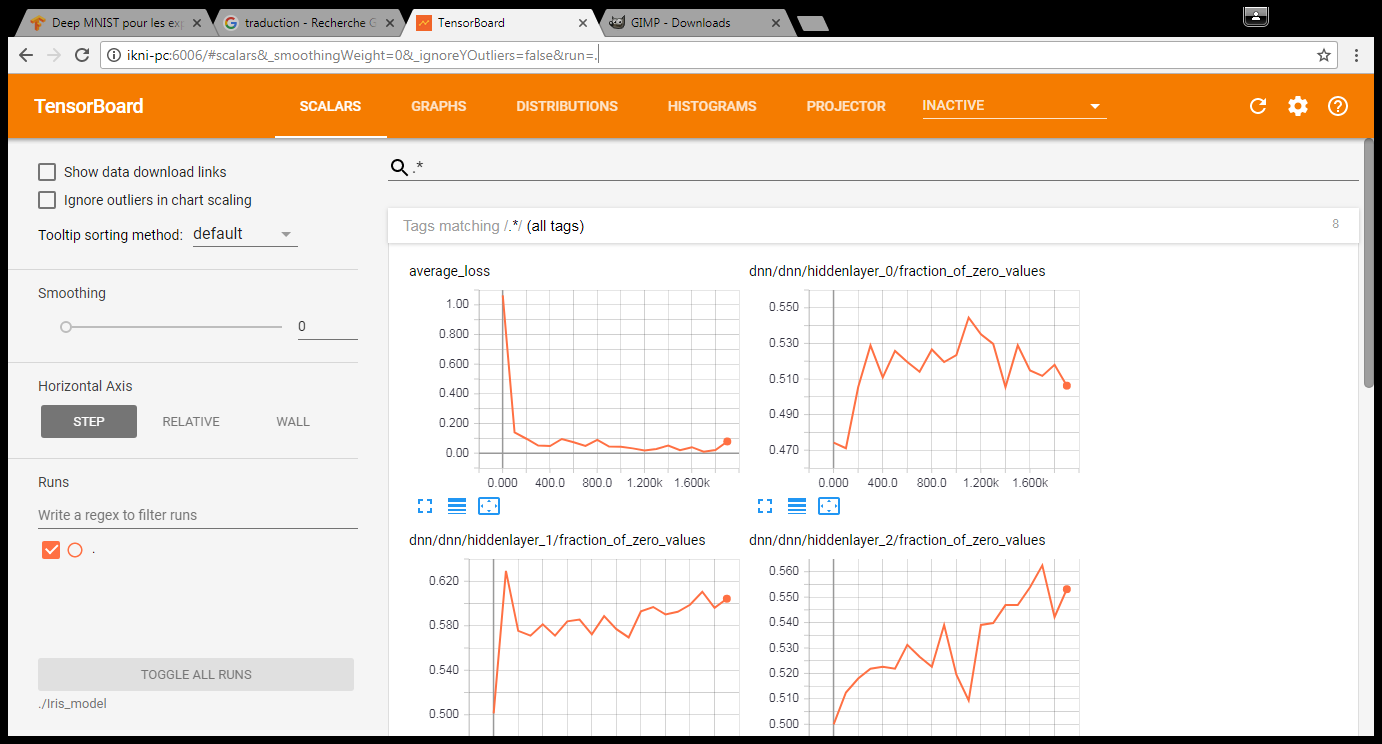
\includegraphics[width=16cm]{./figures/TensorBoardIrisDnn.png} 
\end{center}
\caption{Evolution des paramètres du réseau sur la base IRIS}
\end{figure}

\begin{figure}[H]

\begin{center}
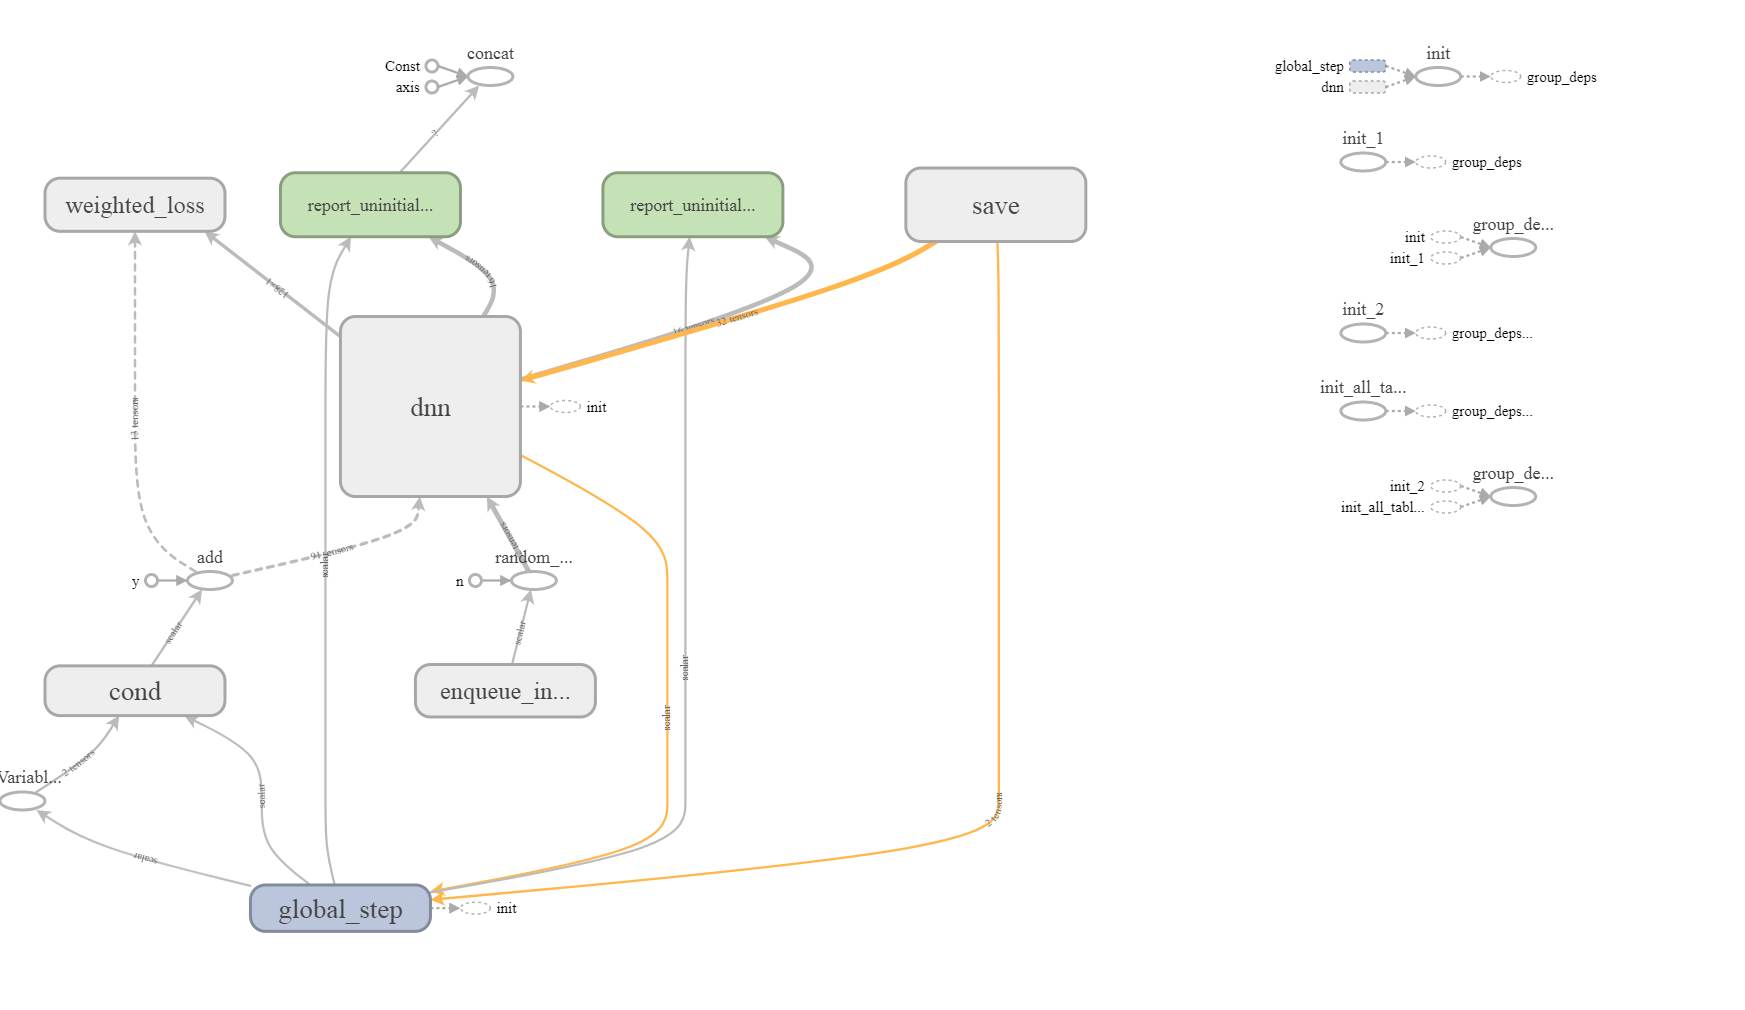
\includegraphics[width=10cm]{./figures/graphIrisDNN.png} 
\end{center}
\caption{Graphe de calcul du DNN utilisé sur la base IRIS}
\end{figure}

\end{document}
